%----------------------------------------------------------------------------------------------
%----------------------------------     4. Vektorgeometrie    ---------------------------------
%----------------------------------------------------------------------------------------------
\section{Vektorgeometrie}

Generell gilt auf dieser Zusammenfassung:
\vspace{0.2cm}
		
\begin{tabular}{ll}
	$\vec{p}$ 		& Ortsvektor (Vektor vom Ursprung zu Punkt auf Geraden)			\\
	$\vec{r}$ 		& Richtungsvektor 												\\
    $\vec{n}$ 		& Normalenvektor (4.1)											\\
	$\vec{x}$ 		& Platzhalter für Punkt (auf Ebene / Geraden) $x_1, x_2, x_3$ 	\\
	$s, t, u, v$ 	& Variablen $\in \mathbb{R}$ 
\end{tabular}		


%----------------------------------------------------------------------------------------------
%----------------------------------     4.1 Normalenvektor    ---------------------------------
%----------------------------------------------------------------------------------------------
\subsection{Normalenvektor}		    

Der Normalenvektor $\vec{n}$ einer Geraden / Ebene steht \textbf{senkrecht} auf der Geraden / Ebene.

Der Normalenvektor $\vec{n}$ kann mit dem Vektorprodukt oder dem Skalarprodukt berechnet werden
\vspace{0.2cm}

\noindent\textbf{Vektorprodukt:}
\[
\vec{n} = \vec{r}_1 \times \vec{r}_2
\]
Beispiel:
\[
\begin{pmatrix}1\\2\\3\end{pmatrix}
\times
\begin{pmatrix}2\\1\\0\end{pmatrix}
=
\begin{pmatrix}-3\\6\\-3\end{pmatrix}
\]

\vspace{0.2cm}
\hrule
\vspace{0.2cm}

\noindent\textbf{Normalenvektor mit dem Skalarprodukt:}
\[
\vec n\cdot\vec r_1=0,\qquad \vec n\cdot\vec r_2=0
\]
Gauss-Tableau:
\[
\begin{pmatrix}
1&2&3&|&0\\
2&1&0&|&0
\end{pmatrix}
\sim
\begin{pmatrix}
1&2&3&|&0\\
0&-3&-6&|&0
\end{pmatrix}
\]
\[
y=-2z,\qquad x=z
\]
Mit \(z=1\) folgt:
\[
\boxed{\vec n=\begin{pmatrix}1\\-2\\1\end{pmatrix}}
\]


%----------------------------------------------------------------------------------------------
%----------------------------------     4.2 Ebenen / Geraden    -------------------------------
%----------------------------------------------------------------------------------------------
\subsection{Darstellungsformen von Ebenen / Geraden}	
		
\subsubsection{Koordinatenform}	% unsicher ob korrekt

\begin{center}
	\renewcommand{\arraystretch}{1.4}
	\begin{tabular}{c|c|c}
							& \textbf{Allgemein}											& \textbf{Beispiel}											\\
		\hline
		\textbf{Gerade} 	& $\crd{n_x} \, x_1 + \crd{n_y} \, x_2  = b$ 					& $\crd{5} \, x_1 + \crd{10} \, x_2 = 6 $ 					\\
		\hline
        \textbf{Ebene}	 	& $\crd{n_x} \, x_1 + \crd{n_y} \, x_2 + \crd{n_z} \, x_3 = b$ 	& $\crd{5} \, x_1 + \crd{10} \, x_2 \crd{- 2} \, x_3 = 6 $ 	\\
	\end{tabular}						    
	\renewcommand{\arraystretch}{1}
\end{center}

Die roten Koeffizienten entsprechen den Koordinaten des Normalenvektors. \\
$b$ entspricht dem Abstand der Ebene zum Nullpunkt des Koordinatensystems.
\vspace{0.2cm}
\subsubsection{Parameterform}

Hinweis: In 2 Dimensionen ohne $z$-Koordinate, ansonsten analog wie im Folgenden:
		
$$ \text{Gerade } g: \quad \vec{p} + s \cdot \vec{r} = \begin{pmatrix} p_x \\ p_y \\ p_z \end{pmatrix}+ t \cdot \begin{pmatrix} r_x \\ r_y \\ r_z \end{pmatrix} $$
$$ \text{Ebene } E: \quad \vec{p} + s \cdot \vec{r}_1 + t \cdot \vec{r}_2 = \begin{pmatrix} p_x \\ p_y \\ p_z \end{pmatrix}	+ s \cdot \begin{pmatrix} r_{1,x} \\ r_{1,y} \\ r_{1,z} \end{pmatrix} + t \cdot \begin{pmatrix} r_{2,x} \\ r_{2,y} \\ r_{3,z} \end{pmatrix} $$ 
		

%----------------------------------------------------------------------------------------------
%----------------------     4.3 Hesse'sche Normalform als Darstellungsform    -----------------
%----------------------------------------------------------------------------------------------
\subsection{Hesse'sche Normalform als Darstellungsform}
\label{Hessesche Normalform}

\textbf{In der Hesse'schen Normalform ist der Abstand $\bm{d}$ vom Nullpunkt zur Ebene immer $\bm{d = 1}$} 
\vspace{0.2cm}

\subsubsection{Beispiel Umwandlung in Hessesche Normalform}

\renewcommand{\arraystretch}{1.5}
\begin{tabular}{ll}
	Ebene $E$: 				& $3 x_1 + 8 x_2 - 5 x_3 = 3$ 					\\
	Hesse'sche Normalform: 	& $x_1 + \frac{8}{3} x_2 - \frac{5}{3} x_3 = 1$
\end{tabular}
\renewcommand{\arraystretch}{1}
		

%----------------------------------------------------------------------------------------------
%----------------------------------     4.4 Orthonormalbasis    -------------------------------
%----------------------------------------------------------------------------------------------
\subsection{Orthonormalbasis}
\label{Orthonormalbasis}

In einer Orthonormalbasis stehen alle verschiedenen Basisvektoren
$\vec{b}_i$ senkrecht aufeinander und haben die Länge $1$.

Ausgedrückt mit dem Skalarprodukt bedeutet dies:
\vspace{0.2cm}

\begin{tabular}{ll}
    Orthogonalität: &
    $\vec{b}_i \bullet \vec{b}_j = 0,\quad i \neq j, \quad 0 = 90^\circ$ \\
    Normierung: &
    $\vec{b}_i \bullet \vec{b}_i = 1$
\end{tabular}
\vspace{0.2cm}\\
Zusammengefasst:
\[
\vec{b}_i \bullet \vec{b}_j = \delta_{ij}
\]

\[
\delta_{ij} =
\begin{cases}
1, & i = j,\\
0, & i \neq j.
\end{cases}
\]
\vspace{0.2cm}

\textbf{Vorteil:} Die Koordinaten eines Vektors $\vec{v}$ können
direkt mit dem Skalarprodukt berechnet werden:
\[
v_i = \vec{v} \bullet \vec{b}_i
\]

\columnbreak


%----------------------------------------------------------------------------------------------
%------------------------------------     4.5 Skalarprodukt    --------------------------------
%----------------------------------------------------------------------------------------------
\subsection{Skalarprodukt}

\begin{minipage}[t]{0.4\columnwidth}
	\begin{center}
		\textbf{\myul{2 Dimensionen}}
		\[
		\vec{a} \bullet \vec{b}
		= |\vec{a}| \cdot |\vec{b}| \cdot \cos(\alpha)
		\]
	\end{center}
\end{minipage}
\hfill
\begin{minipage}[t]{0.58\columnwidth}
	\begin{center}
		\textbf{\myul{3 Dimensionen}}
		\[
		\vec{a} \bullet \vec{b}
		=
		a_x b_x + a_y b_y + a_z b_z
		\]
		Komponentenform bei Orthonormalbasis!
	\end{center}
\end{minipage}

\subsubsection{Eigenschaften des Skalarprodukts}

\renewcommand{\arraystretch}{1.3}
\begin{tabular}{ll}
	Linearität:
	& linear in beiden Vektoren (bilinear) \\

	Orthogonalität:
	& $\vec{a} \bullet \vec{b} = 0$ \\

	Länge im Quadrat:
	& $\vec{a} \bullet \vec{a} = |\vec{a}|^2$ \\

	Länge:
	& $|\vec{a}| = \sqrt{\vec{a} \bullet \vec{a}}$ \\

	Als Matrixprodukt:
	& $\vec{a}^{\,T}\vec{b}
	= \vec{a} \bullet \vec{b}
	= \vec{b}^{\,T}\vec{a}$
\end{tabular}
\renewcommand{\arraystretch}{1}


%----------------------------------------------------------------------------------------------
%----------------------------     4.7 Winkel zwischen zwei Vektoren    ------------------------
%----------------------------------------------------------------------------------------------
\subsection{Winkel zwischen zwei Vektoren}

\vspace{0.2cm}
\begin{minipage}[t]{0.50\columnwidth}
	\begin{center}
		\textbf{\myul{Cosinus}}
		\[
		\cos(\alpha)
		=
		\frac{\vec{a}\bullet\vec{b}}
		{|\vec{a}|\cdot|\vec{b}|}
		\]
	\end{center}
\end{minipage}
\hfill
\begin{minipage}[t]{0.5\columnwidth}
	\begin{center}
		\textbf{\myul{Sinus}}
		\[
		\sin(\alpha)
		=
		\frac{|\vec{a}\times\vec{b}|}
		{|\vec{a}|\cdot|\vec{b}|}
		\]
	\end{center}
\end{minipage}

%----------------------------------------------------------------------------------------------
%--------------------------     4.7 Prallel- und Orthagonalkomponente    ----------------------
%----------------------------------------------------------------------------------------------
\subsection{Prallel- und Orthagonalkomponente}

Ein Vektor kann in zwei orthagonale Komponenten aufgeteilt werden
\begin{center}
	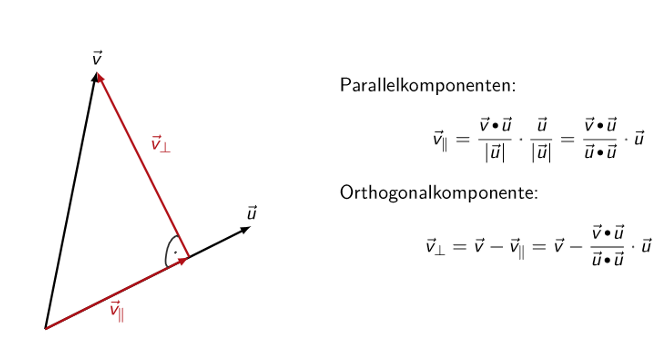
\includegraphics[width=0.65\columnwidth]{images/parallel-orthagonal.PNG}
\end{center}


%----------------------------------------------------------------------------------------------
%-------------------------------------     4.8 Spiegelung    ----------------------------------
%----------------------------------------------------------------------------------------------
\subsection{Spiegelung}

\vspace{-0.2cm}
$$ \text{Der gespiegelte Vektor entspricht } \vec{v'} = \vec{v} - 2 \vec{v}_{\parallel} = \vec{v} - 2 \vec{n} \frac{\vec{n} \bullet \vec{v}}{\vert \vec{n} \vert ^2} $$

\begin{minipage}[c]{0.5\columnwidth} 
	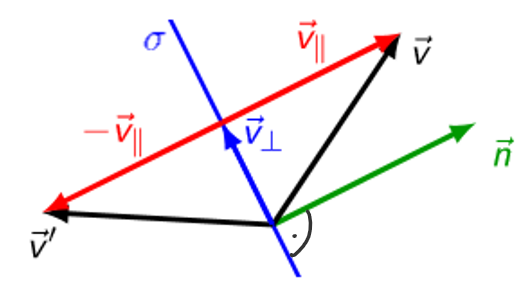
\includegraphics[width=\columnwidth]{images/spiegelung.PNG}
\end{minipage}
\hfill
\begin{minipage}[c]{0.45\columnwidth} 
	Beschreibung der Spiegelnugsmatrix $S$:

	$$ S = I - 2 \frac{1}{\vert \vec{n} \vert ^2} \vec{n} \bullet \vec{n}^t $$ 

	Wenn $\vec{n}$  Länge 1 hat:
	$$ S = I - 2 \vec{n}^0 \bullet \vec{n}^{0 t} $$  	
\end{minipage}						


%----------------------------------------------------------------------------------------------
%------------------------     4.9 Orthagonale Matrix / Orthagonalität    ----------------------
%----------------------------------------------------------------------------------------------
\subsection{Orthagonale Matrix / Orthagonalität}

\textbf{Orthagonal heisst: $A^T A = I$}

\textrightarrow\ Eine orthagonale Matrix ändert das Skalarprodukt nicht.

\subsubsection{Eigenschaften orthagonaler Matritzten}

\begin{minipage}[t]{0.15\columnwidth}
	\begin{itemize}
		\item $A^T A = I$
	\end{itemize}
\end{minipage}
\hfill
\begin{minipage}[t]{0.18\columnwidth}
	\begin{itemize}
		\item $A^{-1} = A^T$
	\end{itemize}
\end{minipage}
\hfill
\begin{minipage}[t]{0.65\columnwidth}
	\begin{itemize}
		\item Wenn $A$ orthagonal ist, dann ist $A^T$ auch orthagonal
	\end{itemize}
\end{minipage}


%----------------------------------------------------------------------------------------------
%-------------------------------     4.10 Hesse'sche Normalform    ----------------------------
%----------------------------------------------------------------------------------------------
\subsection{Hesse'sche Normalform}

\textbf{Berechnung Abstand $\bm{d}$ von Punkt $\vec{x}$ zu Ebene}
\vspace{0.2cm}

\begin{itemize}
    \item Anwendung bei Koordinaten- und Parameterform möglich
    \item $\vec{q}$ entspricht dem Stützvektor der Ebene
\end{itemize}
\vspace{0.2cm}

\subsubsection{Länge des Normalenvektors nicht 1}

\begin{minipage}[t]{0.6\columnwidth}
    \centering\textbf{Koordinatenform}
    \vspace{-0.1cm}
    \[
    d = \frac{|n_x x_1+n_y x_2+n_z x_3-\vec{n}\bullet\vec{q}|}
    {|\vec{n}|}
    \]
\end{minipage}
\hfill
\begin{minipage}[t]{0.38\columnwidth}
    \centering\textbf{Parameterform}
    \vspace{-0.1cm}
    \[
    d = \frac{|\vec{n}\bullet(\vec{x}-\vec{q})|}
    {|\vec{n}|}
    \]
\end{minipage}
\vspace{0.2cm}

\subsubsection{Länge des Normalenvektors ist 1}

\begin{minipage}[t]{0.6\columnwidth}
    \centering\textbf{Koordinatenform}
    \vspace{-0.1cm}
    \[
    d = |n_x x_1+n_y x_2+n_z x_3-\vec{n}\bullet\vec{q}|
    \]
\end{minipage}
\hfill
\begin{minipage}[t]{0.38\columnwidth}
    \centering\textbf{Parameterform}
    \vspace{-0.1cm}
    \[
    d = |\vec{n}\bullet(\vec{x}-\vec{q})|
    \]
\end{minipage}
\vspace{0.5cm}

\textbf{Merke:}
\begin{itemize}
    \item $d \geq 0$ (kürzester Abstand)
    \item Punkt liegt auf Ebene: $d = 0$
    \item $\vec{n}$ steht senkrecht auf der Ebene
    \item Für $|\vec{n}| = 1$ entfällt der Nenner
    \item $\vec{q}$ ist ein beliebiger Punkt auf der Ebene
\end{itemize}
\pagebreak


%----------------------------------------------------------------------------------------------
%--------------------------     4.11 Vektorprodukt (Kreuzprodukt)    --------------------------
%----------------------------------------------------------------------------------------------
\subsection{Vektorprodukt (Kreuzprodukt)}	

\textbf{Nur definiert in 3 Dimensionen!} 

\vspace{0.1cm}

\begin{minipage}[c]{0.45\columnwidth}
	$$\vec{a} \times \vec{b} = 
		\begin{pmatrix}
			a_2 b_3 - a_3 b_2 	\\ 
			a_3 b_1 - a_1 b_3	\\
			a_1 b_2 - a_2 b_1 
		\end{pmatrix}$$
\end{minipage}
\hfill
\begin{minipage}[c]{0.5\columnwidth}
	$\vec{a} \times \vec{b} = -\vec{b} \times \vec{a}$ \\
	$\vec{a} \times \vec{a} = 0$ \\
	$\vec{a} \times (\vec{b} \times \vec{c}) = (\vec{a} \bullet \vec{c}) \, \vec{b} - (\vec{a} \bullet \vec{b}) \, \vec{c}$ \\
	$(\vec{a} \times \vec{b}) \times \vec{c} = (\vec{a} \bullet \vec{c}) \, \vec{b} - (\vec{b} \bullet \vec{c}) \, \vec{a}$
\end{minipage}

\subsubsection{Eigenschaften des Vektorprodukts}

\begin{minipage}[c]{0.68\columnwidth}
	\begin{itemize}
		\item $\vec{a} \times \vec{b}$ ist senkrecht auf $\vec{a}$ und $\vec{b}$ \\
				$( \vec{a} \times \vec{b}) \bullet \vec{a} = \det(\vec{a}, \vec{b}, \vec{a}) = 0$ \\
				$( \vec{a} \times \vec{b}) \bullet \vec{b} = \det(\vec{a}, \vec{b}, \vec{b}) = 0$
		\item $\vert \vec{a} \times \vec{b} \vert$ ist Fläche eines Parallelogramms 
		\item $\vec{a}, \, \vec{b}, \, \vec{a} \times \vec{b}$ bilden ein Rechtssystem
		\item $\vert \vec{a} \times \vec{b} \vert ^2 = (\vec{a} \times \vec{b}) \cdot (\vec{a} \times \vec{b}) = \det(\vec{a}, \, \vec{b}, \, \vec{a} \times \vec{b})$  ist Volumen eines Parallelepipeds
		\item Höhe eines Parallelogramms: $h = \frac{\vert \vec{a} \, \times \, \vec{b} \vert}{ \vert \vec{a} \vert }$
		\item Zwischenwinkel eines Parallelogramms:\\
				$\sin(\alpha) = \frac{h}{\vert \vec{b} \vert} = \frac{\vert \vec{a} \, \times \, \vec{b} \vert}{\vert \vec{a} \vert \bullet \vert \vec{b} \vert}$ 
	\end{itemize}
\end{minipage}
\hfill
\begin{minipage}[c]{0.3\columnwidth}
	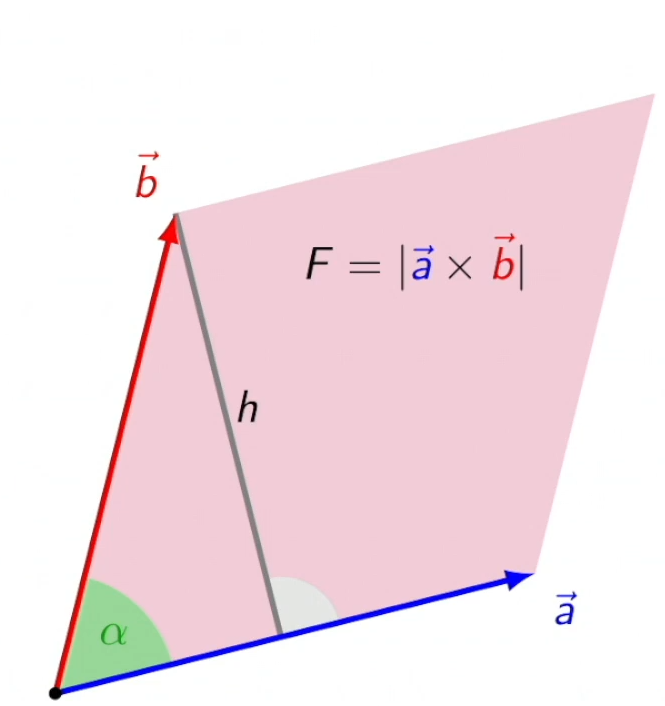
\includegraphics[width=\columnwidth]{images/zwischenwinkel.PNG}
\end{minipage}


%----------------------------------------------------------------------------------------------
%----------------     4.12 Berechnung von Polygonen (Schuhbändelformel)    --------------------
%----------------------------------------------------------------------------------------------
\subsection{Berechnung von Polygonen (Schuhbändelformel)}
		
Die Fläche eines Polygons kann aus Flächen von Dreiecken, also über Determinanten berechnet werden:
\vspace{0.2cm}

\begin{minipage}[c]{0.48\columnwidth}
	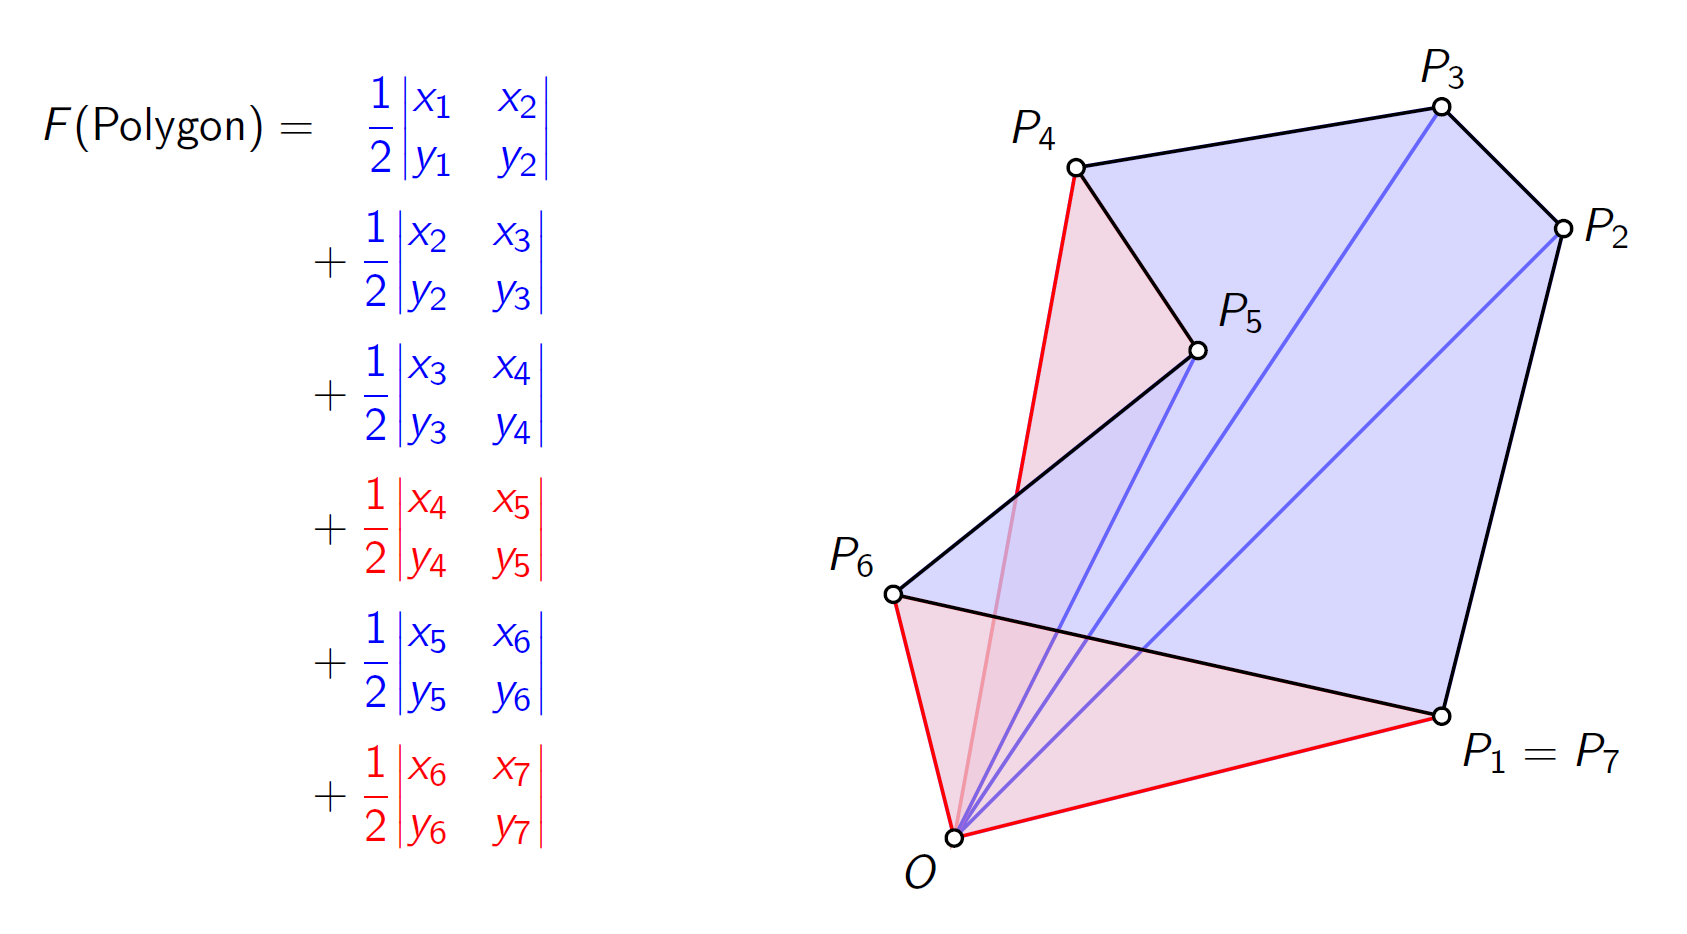
\includegraphics[width=\columnwidth]{images/flaeche-polygon.PNG}
\end{minipage}
\hfill
\begin{minipage}[]{0.48\columnwidth}
	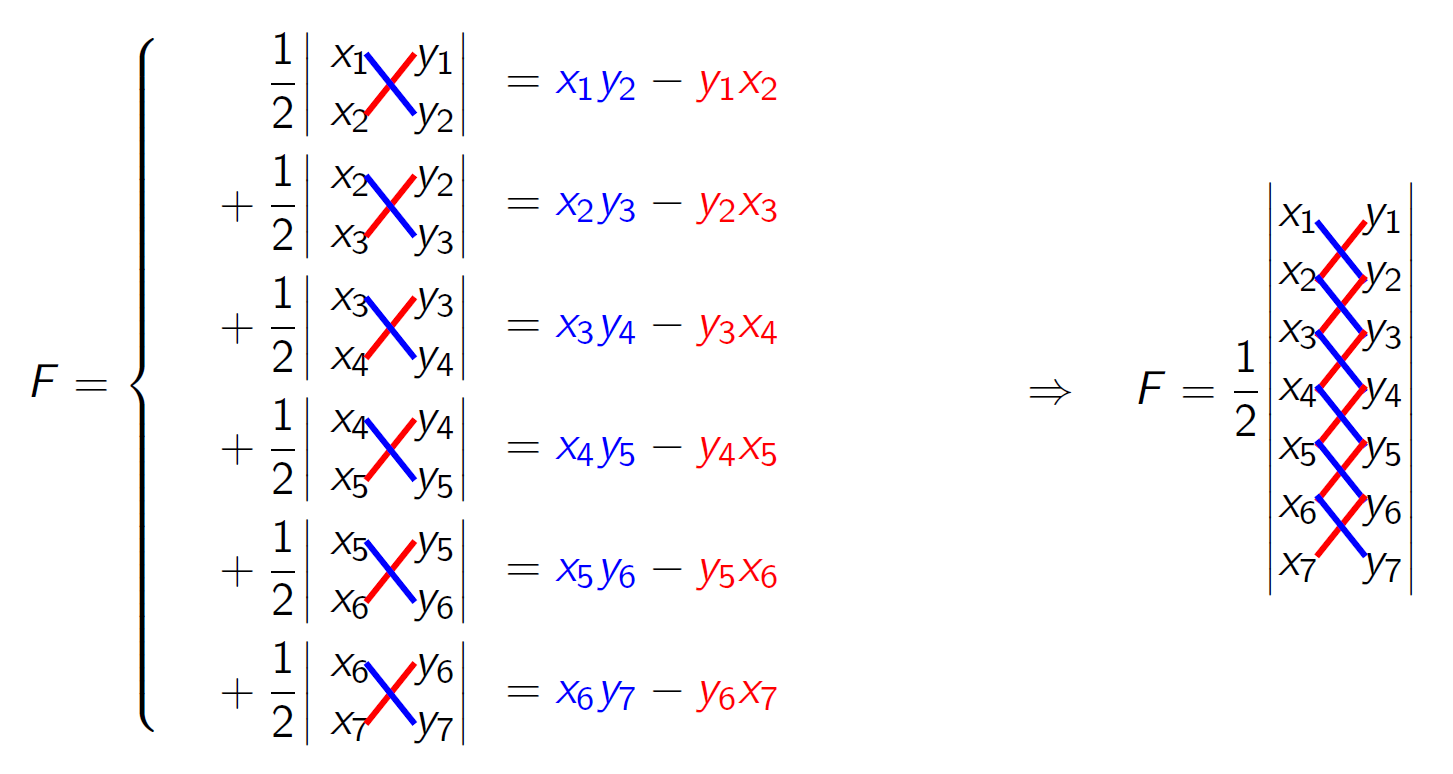
\includegraphics[width=\columnwidth]{images/schuhbaendel.PNG}
\end{minipage}


%----------------------------------------------------------------------------------------------
%-------------------     4.13 Allgemeine Lösung für Schnittprobleme    ------------------------
%----------------------------------------------------------------------------------------------
\subsection{Allgemeine Lösung für Schnittprobleme}	
		
Um ein Schnittproblem zu lösen kann alles in ein Gauss-Tableau geschrieben werden, welches anschliessend gelöst werden kann. 

\begin{minipage}[c]{0.53\columnwidth}
	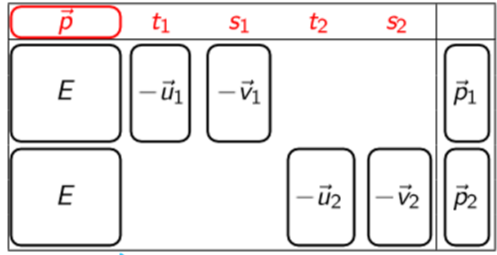
\includegraphics[width=\columnwidth]{images/schnittpunkt-tableau.PNG} 
\end{minipage}
\hfill
\begin{minipage}[c]{0.38\columnwidth}
	\begin{tabular}{ll}
		$E$ 					& Einheitsmatrix  	\\ 
		$\vec{u}, \vec{v}$ 		& Richtungsvektoren \\
		$\vec{p}_1, \vec{p}_1 $ & Stützvektoren 	
	\end{tabular}
\end{minipage}

		
\example{Schnittpunkt von zwei Geraden}

\begin{tabular}{ll}
	$\cbl{\begin{pmatrix} x_1 \\ x_2 \\ x_3 \end{pmatrix} = 
	\begin{pmatrix} 18 \\ -7 \\ 0 \end{pmatrix} + s \cdot 
	\begin{pmatrix} 7 \\ -2 \\ 1\end{pmatrix}}$
	& 
	$\cor{\begin{pmatrix} x_1 \\ x_2 \\ x_3 \end{pmatrix} = 
	\begin{pmatrix} -18 \\ 19 \\ 7 \end{pmatrix} + t \cdot 
	\begin{pmatrix} -3 \\ 4 \\ 2\end{pmatrix}}$ 
\end{tabular}

\vspace{0.2cm}
	
\begin{minipage}[b]{0.5\columnwidth} 
	\begin{tabular}{| c c c c c | c |}
		\hline
		$x_1$ 		& $x_2$ 	& $x_3$ 	& $s$ 			& $t$ 			& 				\\
		\hline	
		$\cbl{1}$ 	& $\cbl{0}$ & $\cbl{0}$	& $\cbl{-7}$ 	& $\cbl{0}$		& $\cbl{18}$	\\
		$\cbl{0}$ 	& $\cbl{1}$ & $\cbl{0}$	& $\cbl{2}$		& $\cbl{0}$		& $\cbl{-7}$ 	\\
		$\cbl{0}$ 	& $\cbl{0}$ & $\cbl{1}$	& $\cbl{-1}$ 	& $\cbl{0}$		& $\cbl{0}$ 	\\
		$\cor{1}$ 	& $\cor{0}$ & $\cor{0}$	& $\cor{0}$		& $\cor{3}$		& $\cor{-18}$ 	\\
		$\cor{0}$ 	& $\cor{1}$ & $\cor{0}$	& $\cor{0}$		& $\cor{-4}$ 	& $\cor{19}$ 	\\
		$\cor{0}$ 	& $\cor{0}$ & $\cor{1}$	& $\cor{0}$		& $\cor{-2}$ 	& $\cor{7}$ 	\\
		\hline
	\end{tabular}		
\end{minipage}
\hfill
\begin{minipage}[b]{.45\columnwidth} 
	% Es wurden Farben gewünscht...
	\begin{tabular}{| c c c c c | c |}
		\hline
		$x_1$ 	& $x_2$ & $x_3$ & $s$ & $t$ & 							\\
		\hline
		$1$ 	& $0$ 	& $0$	& $0$ & $0$ & $\cbl{-3}$ 				\\
		$0$ 	& $1$ 	& $0$	& $0$ & $0$ & $\cor{-1}$ 				\\
		$0$ 	& $0$ 	& $1$	& $0$ & $0$ & $\cgn{-3}$ 				\\
		$0$ 	& $0$ 	& $0$	& $1$ & $0$ & $\cvt{-3}$ 	\\
		$0$ 	& $0$ 	& $0$	& $0$ & $1$ & $\textcolor{teal}{-5}$ 	\\
		$0$ 	& $0$ 	& $0$	& $0$ & $0$ & $0$ 						\\
		\hline
	\end{tabular}		
\end{minipage}		
	
\vspace{0.2cm}

Schnittpunkt: ($\cbl{-3}$ $\vert$ $\cor{-1}$ $\vert$ $\cgn{-3}$) \quad
$s = \cvt{-3}$ \quad $t = \textcolor{teal}{-5}$	
	
\vspace{0.4cm}

\example{Durchstosspunkt Gerade durch Ebene}

\begin{tabular}{ll}
	$\cbl{\begin{pmatrix} x_1 \\ x_2 \\ x_3 \end{pmatrix} = 
	\begin{pmatrix} 0 \\ 0 \\ 1 \end{pmatrix} + s \cdot 
	\begin{pmatrix} 1 \\ 1 \\ -1\end{pmatrix}}$
	&
	$\cor{\begin{pmatrix} x_1 \\ x_2 \\ x_3 \end{pmatrix} = 
	\begin{pmatrix} 0 \\ 0 \\ 0 \end{pmatrix} + u \cdot 
	\begin{pmatrix} 1 \\ 0 \\ 1\end{pmatrix} + v \cdot 
	\begin{pmatrix} 0 \\ 1 \\ 1\end{pmatrix}}$
\end{tabular}

\vspace{0.2cm}

\begin{minipage}[b]{0.49\columnwidth}
	\begin{tabular}{| c c c c c c | c |}
		\hline
		$x_1$ 		& $x_2$ 	& $x_3$ 	& $s$ 			& $u$ 			& $v$ 			& 			\\
		\hline
		$\cbl{1}$ 	& $\cbl{0}$	& $\cbl{0}$	& $\cbl{-1}$	& $\cbl{0}$		& $\cbl{0}$		& $\cbl{0}$	\\
		$\cbl{0}$ 	& $\cbl{1}$	& $\cbl{0}$	& $\cbl{-1}$	& $\cbl{0}$		& $\cbl{0}$		& $\cbl{0}$	\\
		$\cbl{0}$ 	& $\cbl{0}$	& $\cbl{1}$	& $\cbl{1}$		& $\cbl{0}$		& $\cbl{0}$		& $\cbl{1}$	\\
		$\cor{1}$ 	& $\cor{0}$	& $\cor{0}$	& $\cor{0}$		& $\cor{-1}$	& $\cor{0}$		& $\cor{0}$	\\
		$\cor{0}$ 	& $\cor{1}$	& $\cor{0}$	& $\cor{0}$		& $\cor{0}$		& $\cor{-1}$	& $\cor{0}$	\\
		$\cor{0}$ 	& $\cor{0}$	& $\cor{1}$	& $\cor{0}$		& $\cor{-1}$	& $\cor{-1}$	& $\cor{0}$	\\
		\hline
	\end{tabular}	
\end{minipage}
\hfill
\begin{minipage}[b]{0.48\columnwidth}
	% Es wurden Farben gewünscht...
	\renewcommand{\arraystretch}{1.2}
	\begin{tabular}{| c c c c c c | c |}
		\hline
		$x_1$ 	& $x_2$	& $x_3$	& $s$ 	& $u$ & $v$ & 									\\
		\hline
		$1$ 	& $0$ 	& $0$ 	& $0$ 	& $0$ & $0$ & $\cbl{\frac{1}{3}}$ 				\\
		$0$ 	& $1$ 	& $0$ 	& $0$ 	& $0$ & $0$ & $\cor{\frac{1}{3}}$ 				\\
		$0$ 	& $0$ 	& $1$ 	& $0$ 	& $0$ & $0$ & $\cgn{\frac{2}{3}}$ 				\\
		$0$ 	& $0$ 	& $0$ 	& $1$ 	& $0$ & $0$ & $\cvt{\frac{1}{3}}$ \\
		$0$ 	& $0$ 	& $0$ 	& $0$ 	& $1$ & $0$ & $\textcolor{teal}{\frac{1}{3}}$ 	\\
		$0$ 	& $0$ 	& $0$ 	& $0$ 	& $0$ & $1$ & $\crd{\frac{1}{3}}$ 				\\
		\hline
	\end{tabular}	
	\renewcommand{\arraystretch}{1}	
\end{minipage}

\vspace{0.2cm}

Durchstosspunkt: ($\cbl{\frac{1}{3}} \vert \cor{\frac{1}{3}} \vert \cgn{\frac{2}{3}}$)
\quad $s = \cvt{\frac{1}{3}}$ \quad $u = \textcolor{teal}{\frac{1}{3}}$ \quad $v = \crd{\frac{1}{3}}$	
					
\columnbreak
\example{Schnittgerade von 2 Ebenen}		    					

\begin{tabular}{ll}
	$\cbl{\begin{pmatrix} x_1 \\ x_2 \\ x_3 \end{pmatrix} = 
	\begin{pmatrix} 6 \\ 4 \\ 7 \end{pmatrix} 
	+ s \cdot \begin{pmatrix} 3 \\ -2 \\ 2\end{pmatrix} 
	+ t \cdot \begin{pmatrix} -5 \\ 3 \\ -7\end{pmatrix}}$
	&
	$\cor{\begin{pmatrix} x_1 \\ x_2 \\ x_3 \end{pmatrix} = 
	\begin{pmatrix} 2 \\ 2 \\ 4 \end{pmatrix} 
	+ u \cdot \begin{pmatrix} 4 \\ 11 \\ 0\end{pmatrix} 
	+ v \cdot \begin{pmatrix} -1 \\ 1 \\ 3\end{pmatrix}}$
\end{tabular}

\vspace{0.2cm}

\begin{tabular}{| c c c c c c c | c |}
\hline
$x_1$ 		& $x_2$ 	& $x_3$ 	& $s$ 			& $t$ 			& $u$ 			& $v$ 			&  			\\
\hline
$\cbl{1}$ 	& $\cbl{0}$ & $\cbl{0}$ & $\cbl{-3}$	& $\cbl{5}$		& $\cbl{0}$ 	& $\cbl{0}$ 	& $\cbl{6}$	\\
$\cbl{0}$ 	& $\cbl{1}$ & $\cbl{0}$ & $\cbl{2}$ 	& $\cbl{-3}$	& $\cbl{0}$ 	& $\cbl{0}$ 	& $\cbl{4}$	\\
$\cbl{0}$ 	& $\cbl{0}$ & $\cbl{1}$ & $\cbl{-2}$ 	& $\cbl{7}$		& $\cbl{0}$ 	& $\cbl{0}$ 	& $\cbl{7}$ \\
$\cor{1}$ 	& $\cor{0}$ & $\cor{0}$ & $\cor{0}$ 	& $\cor{0}$		& $\cor{-4}$ 	& $\cor{1}$ 	& $\cor{2}$ \\
$\cor{0}$ 	& $\cor{1}$ & $\cor{0}$ & $\cor{0}$		& $\cor{0}$		& $\cor{-11}$	& $\cor{-1}$	& $\cor{2}$ \\
$\cor{0}$ 	& $\cor{0}$ & $\cor{1}$ & $\cor{0}$ 	& $\cor{0}$		& $\cor{0}$ 	& $\cor{-3}$	& $\cor{4}$ \\
\hline
\end{tabular}		
	

\begin{minipage}[b]{0.55\columnwidth}
	% Es wurden Farben gewünscht...
	\renewcommand{\arraystretch}{1.2}
	\begin{tabular}{| c c c c c c c | c |}
		\hline
		$x_1$ 	& $x_2$ & $x_3$	& $s$ 	& $t$ 	& $u$ 	& $v$ 						& 						\\
		\hline
		$1$ 	& $0$	& $0$	&	$0$ &	$0$	&	$0$	& $\cvt{-1}$ 				& $\cbl{\frac{10}{3}}$	\\
		$0$ 	& $1$	& $0$	&	$0$ &	$0$	&	$0$	& $\textcolor{teal}{1}$ 	& $\cor{\frac{17}{3}}$	\\
		$0$ 	& $0$	& $1$	&	$0$ &	$0$	&	$0$	& $\crd{3}$ 				& $\cgn{4}$				\\
		$0$ 	& $0$	& $0$	&	$1$ &	$0$	&	$0$	& $2$ 						& $-\frac{1}{3}$		\\
		$0$ 	& $0$	& $0$	&	$0$ &	$1$	&	$0$	& $1$ 						& $\frac{1}{3}$			\\
		$0$ 	& $0$	& $0$	&	$0$ &	$0$	&	$1$	& $0$ 						& $\frac{1}{3}$			\\
		\hline
	\end{tabular}	
	\renewcommand{\arraystretch}{1}	
\end{minipage}
\hfill
\begin{minipage}[b]{0.44\columnwidth}
	Schnittgerade: $\begin{pmatrix} x_1 \\ x_2 \\ x_3 \end{pmatrix} = 
					\begin{pmatrix} \cbl{\frac{10}{3}} \\ \cor{\frac{17}{3}} \\ \cgn{4} \end{pmatrix}
					+ v \cdot \begin{pmatrix} \cvt{-1} \\ \textcolor{teal}{1} \\ \crd{3} \end{pmatrix} $
\end{minipage}


%----------------------------------------------------------------------------------------------
%---------------------------     4.14 Orthonormalisierung    ----------------------------------
%----------------------------------------------------------------------------------------------
\subsection{Orthonormalisierung}
		
Beschreibt, wie man von einer beliebigen Basis zu einer Orthonormalbasis kommt \\		
Orthonormalbasis: siehe Abschnitt \ref{Orthonormalbasis}
		

\subsubsection{Gram-Schmidtsches Orthonormalisierungsverfahren}

Basisvektoren $\vec{a}_1$, $\vec{a}_2$ und $\vec{a}_3$ sind nicht orthagonal. Sie sollen
orthagonalisiert werden und durch die Vektoren $\vec{b}_1$, $\vec{b}_2$ und $\vec{b}_3$ 
ausgedrückt werden:
\vspace{0.2cm}
		
\begin{tabular}{lll}
	$\vec{b}_1$ = $\frac{\vec{a}_1}{\vert \vec{a}_1 \vert}$ &
	$\vec{b}_2$  = $\frac{\vec{a}_2 - ( \vec{a}_2 \bullet \vec{b}_1 ) \vec{b}_1}{\vert \vec{a}_2 - ( \vec{a}_2 \bullet \vec{b}_1 ) \vec{b}_1 \vert}$ &
	$\vec{b}_3$ = $\frac{\vec{a}_3 - ( \vec{a}_3 \bullet \vec{b}_1 ) \vec{b}_1 - ( \vec{a}_3 \bullet \vec{b}_2 ) \vec{b}_2}  {\vert \vec{a}_3 - ( \vec{a}_3 \bullet \vec{b}_1 ) \vec{b}_1 - ( \vec{a}_3 \bullet \vec{b}_2 ) \vec{b}_2 \vert}$ 
\end{tabular}

\vspace{0.2cm}
\textrightarrow\ Kann beliebig weitergeführt werden	


%----------------------------------------------------------------------------------------------
%-------------------------------     4.15 Least Squares    ------------------------------------
%----------------------------------------------------------------------------------------------
\subsection{Least Squares -- Überbestimmtes Gleichungssystem}

Ein Gleichungssystem mit \textbf{mehr Gleichungen als Unbekannten} ist im allgemeinen nicht lösbar. \\	
Wir suchen also eine Lösung, welche \textbf{am 'wenigsten falsch'} ist bzw. $\vert A \cdot \vec{x} - \vec{b} \vert$ möglichst klein ist. 
			

\example{Least Squares}

Es sind Punkte gegeben: $(x_i \, , y_i)$ Die Unbekannten sind \crd{rot} eingefärbt \\
Die gegebenen Punkte sollen durch eine Gerade mit kleinstmöglichem Fehler approximiert werden. \\
Finde die \crd{unbekannten Parameter} der Geradengleichung $\crd{a} \cdot x_i + \crd{b}$ 

\vspace{0.2cm}

\begin{minipage}[c]{0.48\columnwidth}
	$$ \underbrace{\begin{pmatrix}
			x_1 & 1 \\
			x_2 & 1 \\
			\vdots & \vdots \\
			x_n & 1
		\end{pmatrix}}_{\substack{A}} 
		\cdot
		\underbrace{\begin{pmatrix}
			\crd{a} \\
			\crd{b}
		\end{pmatrix}}_{\substack{\crd{\vec{x}}}} 
		= 
		\underbrace{\begin{pmatrix}
			y_1 \\
			y_2 \\
			\vdots \\
			y_n
		\end{pmatrix}}_{\substack{\vec{b}}} $$
\end{minipage}
\hfill
\begin{minipage}[c]{0.48\columnwidth}
	\center{\textrightarrow\ Least Squares}
	$$ \crd{\vec{x}} = (A^t A)^{-1} A^t \vec{b} $$
\end{minipage}

\vspace{0.2cm}
\textbf{Nichtlineare Teile (z.B. $\bm{d^2}$) können einfach neu benannt weden ($\bm{d^2 = m}$) und in das Verfahren eingesetzt werden.} \\
Sobald eine lineare Lösung gefunden ist kann der nichtlineare Teil berechnet werden.


%----------------------------------------------------------------------------------------------
%------------------------------------     4.16 Kreis    ---------------------------------------
%----------------------------------------------------------------------------------------------
\subsection{Kreis}		
		
\subsubsection{Kreisgleichungen}

\begin{tabular}{ll}
	Vektorgleichung: 		& $(\vec{p} - \vec{m})^2 = r^2$		\\
	Koordinatengleichung: 	& $(x- m_x)^2 + (y-m_y)^2 = r^2$
\end{tabular}
		
\vspace{0.2cm}
Die Koeffizienten vor $x$ und $y$ entsprechen Koordinatenmittelpunkt: 

$x^2 - 2 \crd{m_x} x + m_x^2 + y^2 - 2 \crd{m_y} y + m_y^2 = r^2 $ 
\begin{center}
	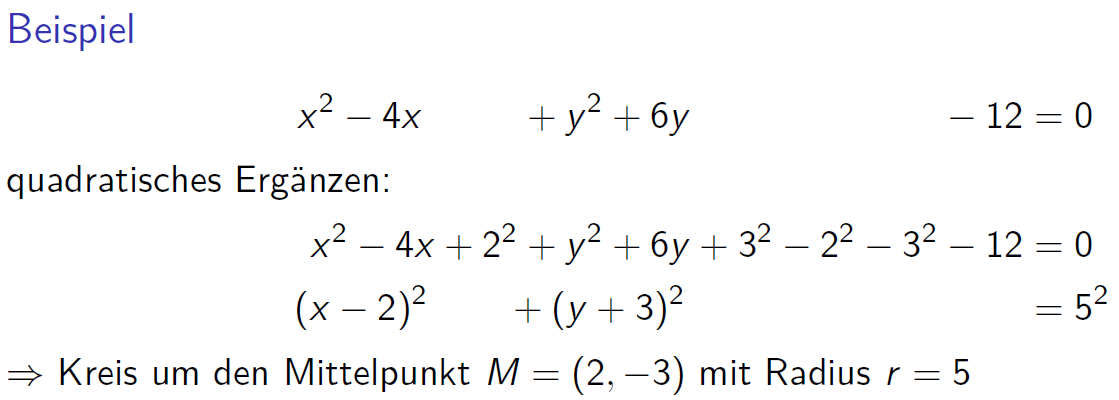
\includegraphics[width=0.8\columnwidth]{images/kreisgleichung.PNG} 
\end{center}

\subsubsection{Thales-Kreis}
		
\begin{minipage}[c]{0.45\columnwidth} 
	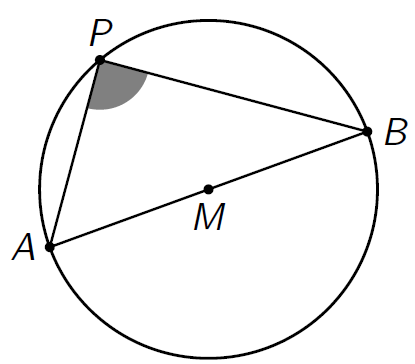
\includegraphics[width=0.7\columnwidth]{images/thales-kreis.PNG}
\end{minipage}
\hfill
\begin{minipage}[c]{0.5\columnwidth} 
	\begin{center}
		\myul{\textbf{Thales-Kreis}}
	\end{center}
	$$ \left( \vec{p} - \frac{\vec{a} + \vec{b}}{2} \right) ^2 = \left( \frac{\vec{a} - \vec{b}}{2} \right) ^2 = r^2 $$
\end{minipage}	

\subsubsection{Durchstosspunkt Gerade-Kreis}

\begin{center}
	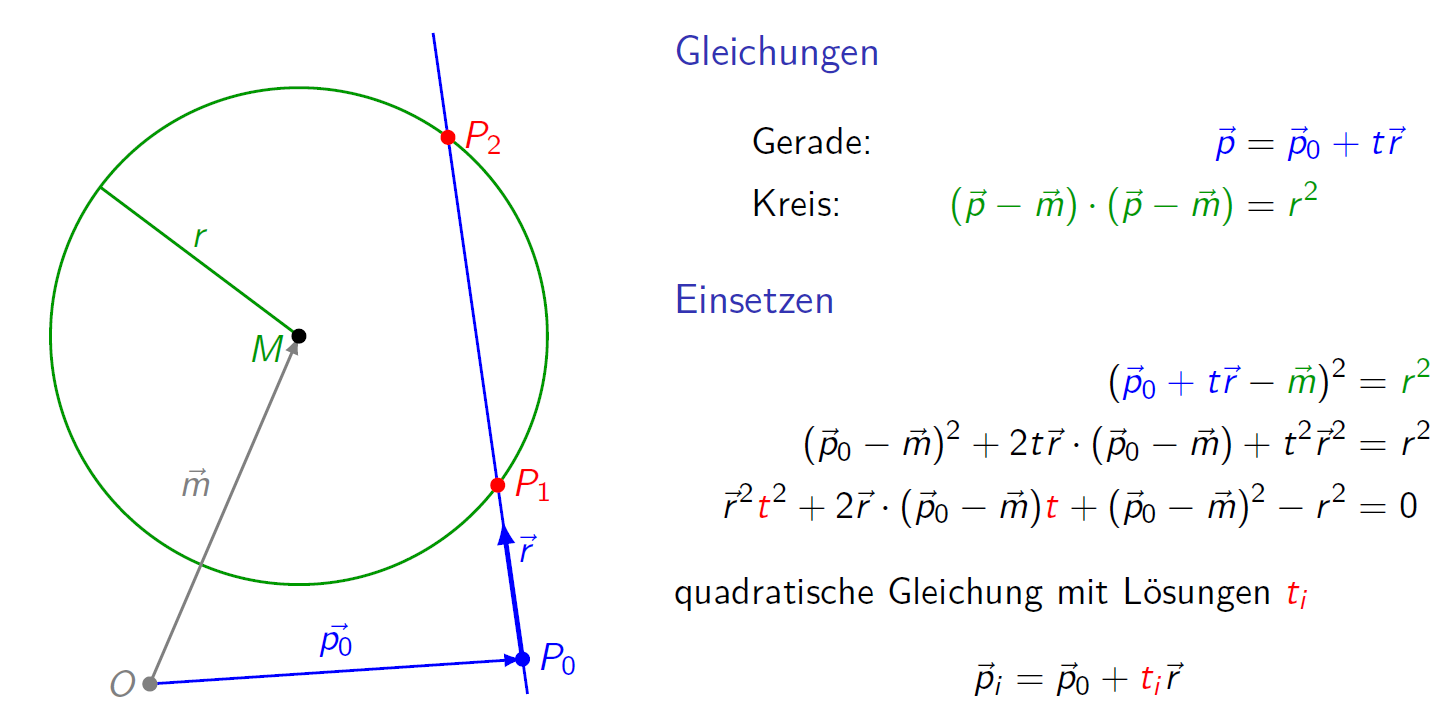
\includegraphics[width=0.7\columnwidth]{images/durchstosspunkt-gerade-kreis.PNG}
\end{center}

\vspace{0.05cm}
	
\subsubsection{Tangente an Kreis}

\begin{center}
	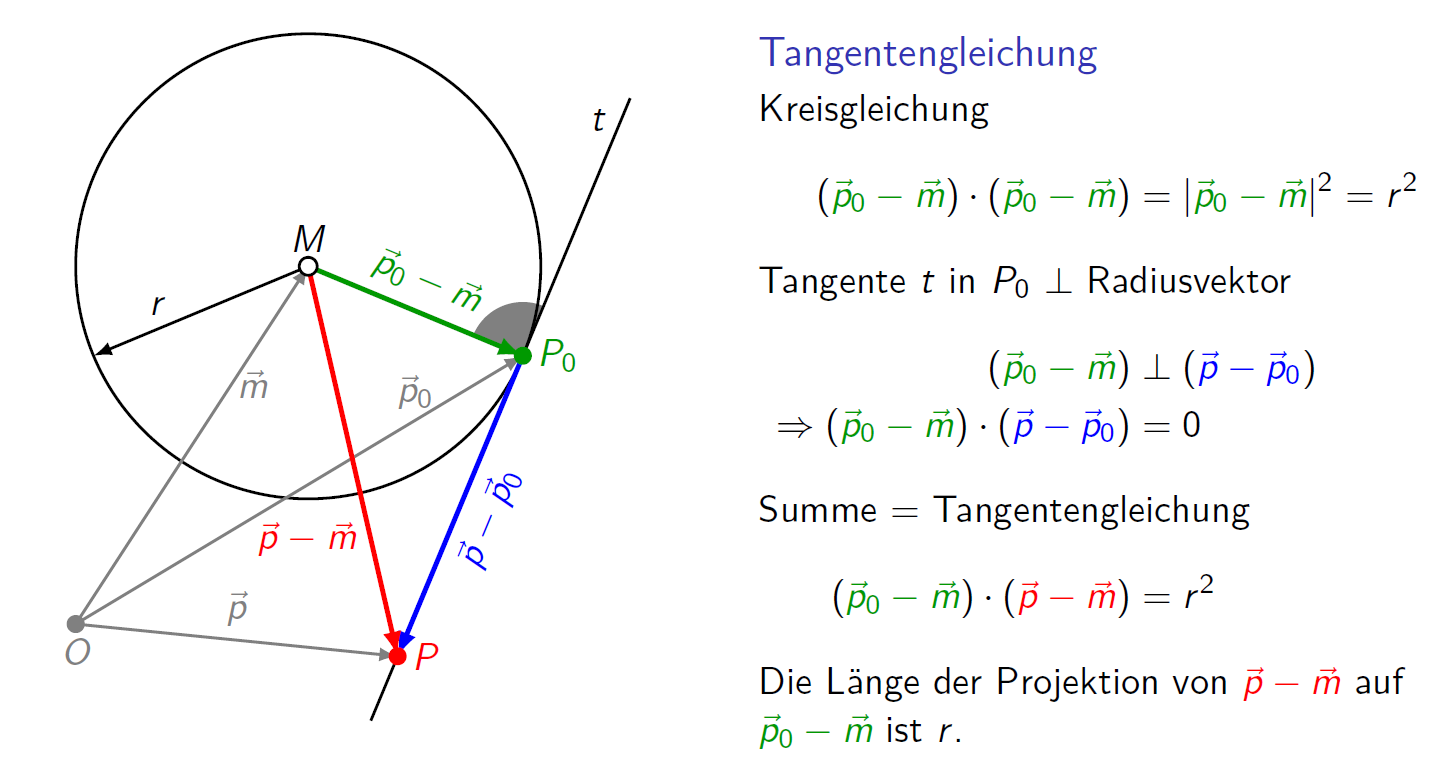
\includegraphics[width=0.7\columnwidth]{images/kreis-tangente.PNG}	
\end{center}


%----------------------------------------------------------------------------------------------
%------------------------------------     4.17 Kugel    ---------------------------------------
%----------------------------------------------------------------------------------------------
\subsection{Kugel}

\subsubsection{Kugelgleichungen}

\begin{tabular}{ll}
	Vektorgleichung: 		& $(\vec{p} - \vec{m})^2 = r^2$						\\
	Koordinatengleichung: 	& $(x - m_x)^2 + (y - m_y)^2 + (z - m_z)^2 = r^2$
\end{tabular}
		


\subsubsection{Formeln zur Kugel}

\begin{center}
	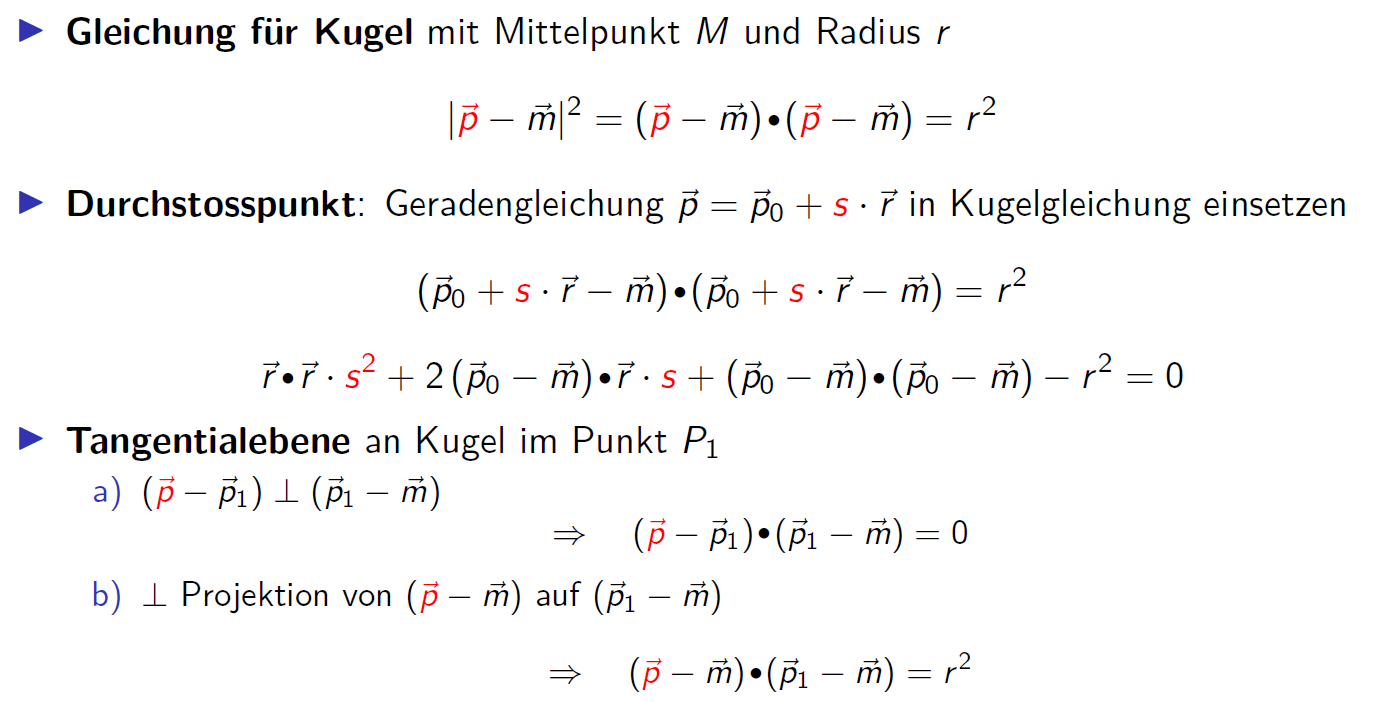
\includegraphics[width=0.8\columnwidth]{images/kugel.PNG}	
\end{center}


%----------------------------------------------------------------------------------------------
%-------------------------------     4.18 Abstandsprobleme    ---------------------------------
%----------------------------------------------------------------------------------------------
\subsection{Abstandsprobleme}
	
\subsubsection{Abstand Punkt-Ebene}

Berechnung mittels Hesse'scher Normalform \textrightarrow\ Siehe Abschnitt \ref{Hessesche Normalform}


	
\subsubsection{Abstand Punkt-Gerade}

Der Abstand $h$ zwischen der Geraden $g$ und dem Punkt $Q$ entspricht dem Lot zur Geraden $g$ durch $Q$

		
\begin{minipage}{0.3\columnwidth}
	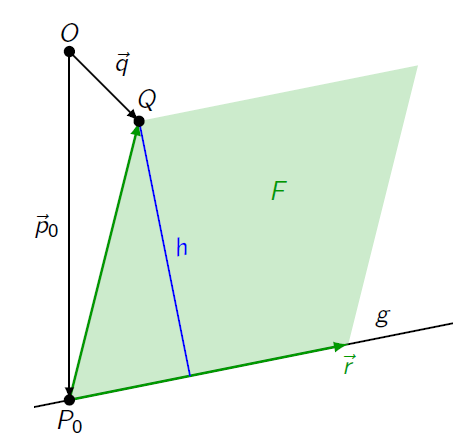
\includegraphics[width=\columnwidth]{images/punkt-gerade.PNG}
\end{minipage}
\hfill
\begin{minipage}{0.6\columnwidth}
	\begin{center}
		\textbf{Gerade in Paramterdarstellung}
	\end{center}
	$$ \vec{p} = \vec{p}_0 + t \cdot \vec{r}$$ 

	\begin{center}
		\textbf{Abstand zwischen Punkt und Gerade}
	\end{center}
	$$  h = \frac{F}{|\vec{r}| } =  \frac{r \times ( |\vec{q} - \vec{p}_0 |)}{| \vec{r} |} $$
\end{minipage}



\subsubsection{Abstand windschiefer Geraden in 3D} 
	
\textbf{Vorausetzung:} Zwei Geraden in Parameterdarstellung, die sich nicht schneiden und nicht parallel sind:
$\vec{p} = \vec{p}_0 + t \cdot \vec{r}_1$ und $\vec{q} = \vec{q}_0 + 2 \vec{r}_2$ 
$$ \text{Abstand:} \quad d = (\vec{q}_0 -\vec{p}_0) \bullet \frac{\vec{r}_1 \times \vec{r}_2}{\vert \vec{r}_1 \times \vec{r}_2 \vert} $$

	
\subsubsection{Minimaler Abstand}

\begin{center}
	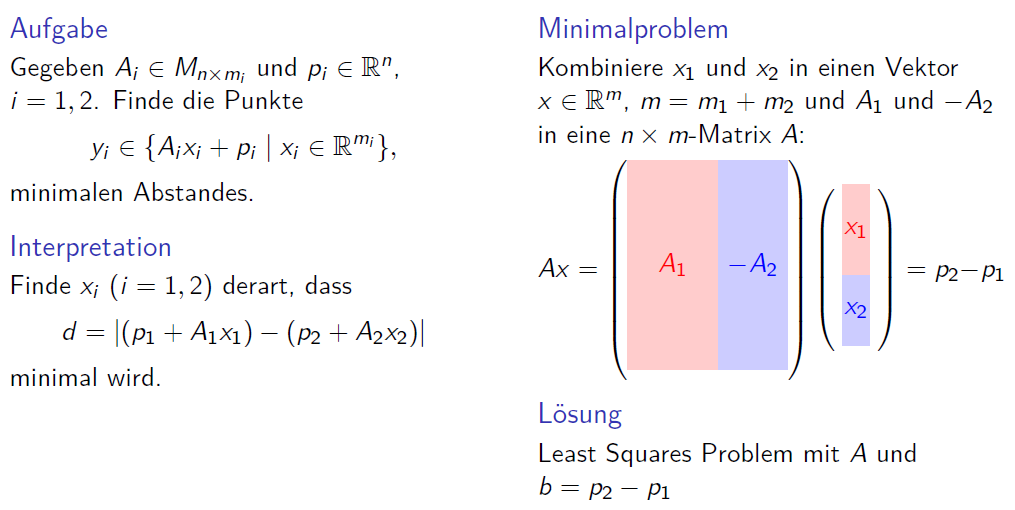
\includegraphics[width=0.7\columnwidth]{images/minimaler-abstand.PNG}	
\end{center}
